%% ----------------------------------------------------------------
%% Project.tex
%% ---------------------------------------------------------------- 

\documentclass{ecsproject}     % Use the Project Style
\usepackage{titlesec}
\titleformat{\chapter}
  {\normalfont\huge\bfseries}{\ \thechapter.}{20pt}{\huge}
\graphicspath{{figures/}}   % Location of your graphics files
\usepackage{natbib}            % Use Natbib style for the refs.
\hypersetup{colorlinks=false}   % Set to false for black/white printing

%% ----------------------------------------------------------------
\begin{document}
\frontmatter
\title      {Folidity - Safe Functional Smart Contract Language}
\authors    {\texorpdfstring
             {\href{mailto:gn2g21@soton.ac.uk}{German Nikolishin}}
             {German Nikolishin}
            }
\addresses  {\groupname\\\deptname\\\univname}
\date       {\today}
\subject    {}
\keywords   {}
\supervisor {\texorpdfstring
            {\href{mailto:gn2g21@soton.ac.uk}{Prof. Vladimiro Sassone}}
            {Prof. Vladimiro Sassone}
}
\examiner   {Dr Butthead}
\degree     {BSc Computer Science}
\maketitle
\tableofcontents
% \listoffigures
% \listoftables
% \lstlistoflistings
% \listofsymbols{ll}{$w$ & The weight vector}
% \acknowledgements{Thanks to no one.}
% \dedicatory{To \dots}
\mainmatter
%% ----------------------------------------------------------------

\chapter{Introduction} \label{Chapter:Introduction}
You probably found all the files from \cite{test_this_nodate}.
\tref{Table:tabex} illustrates the results of my work.
\begin{table}[!htb]
  \centering
  \begin{tabular}{cc}
  \toprule
  \textbf{Training Error} & \textbf{Testing Error}\\
  \midrule
  0 & $\infty$\\
  \bottomrule
  \end{tabular}
  \caption{The Results}
  \label{Table:tabex}
\end{table}

\fref{Figure:figex} shows why this is the case.
\begin{figure}[!htb]
  \centering
  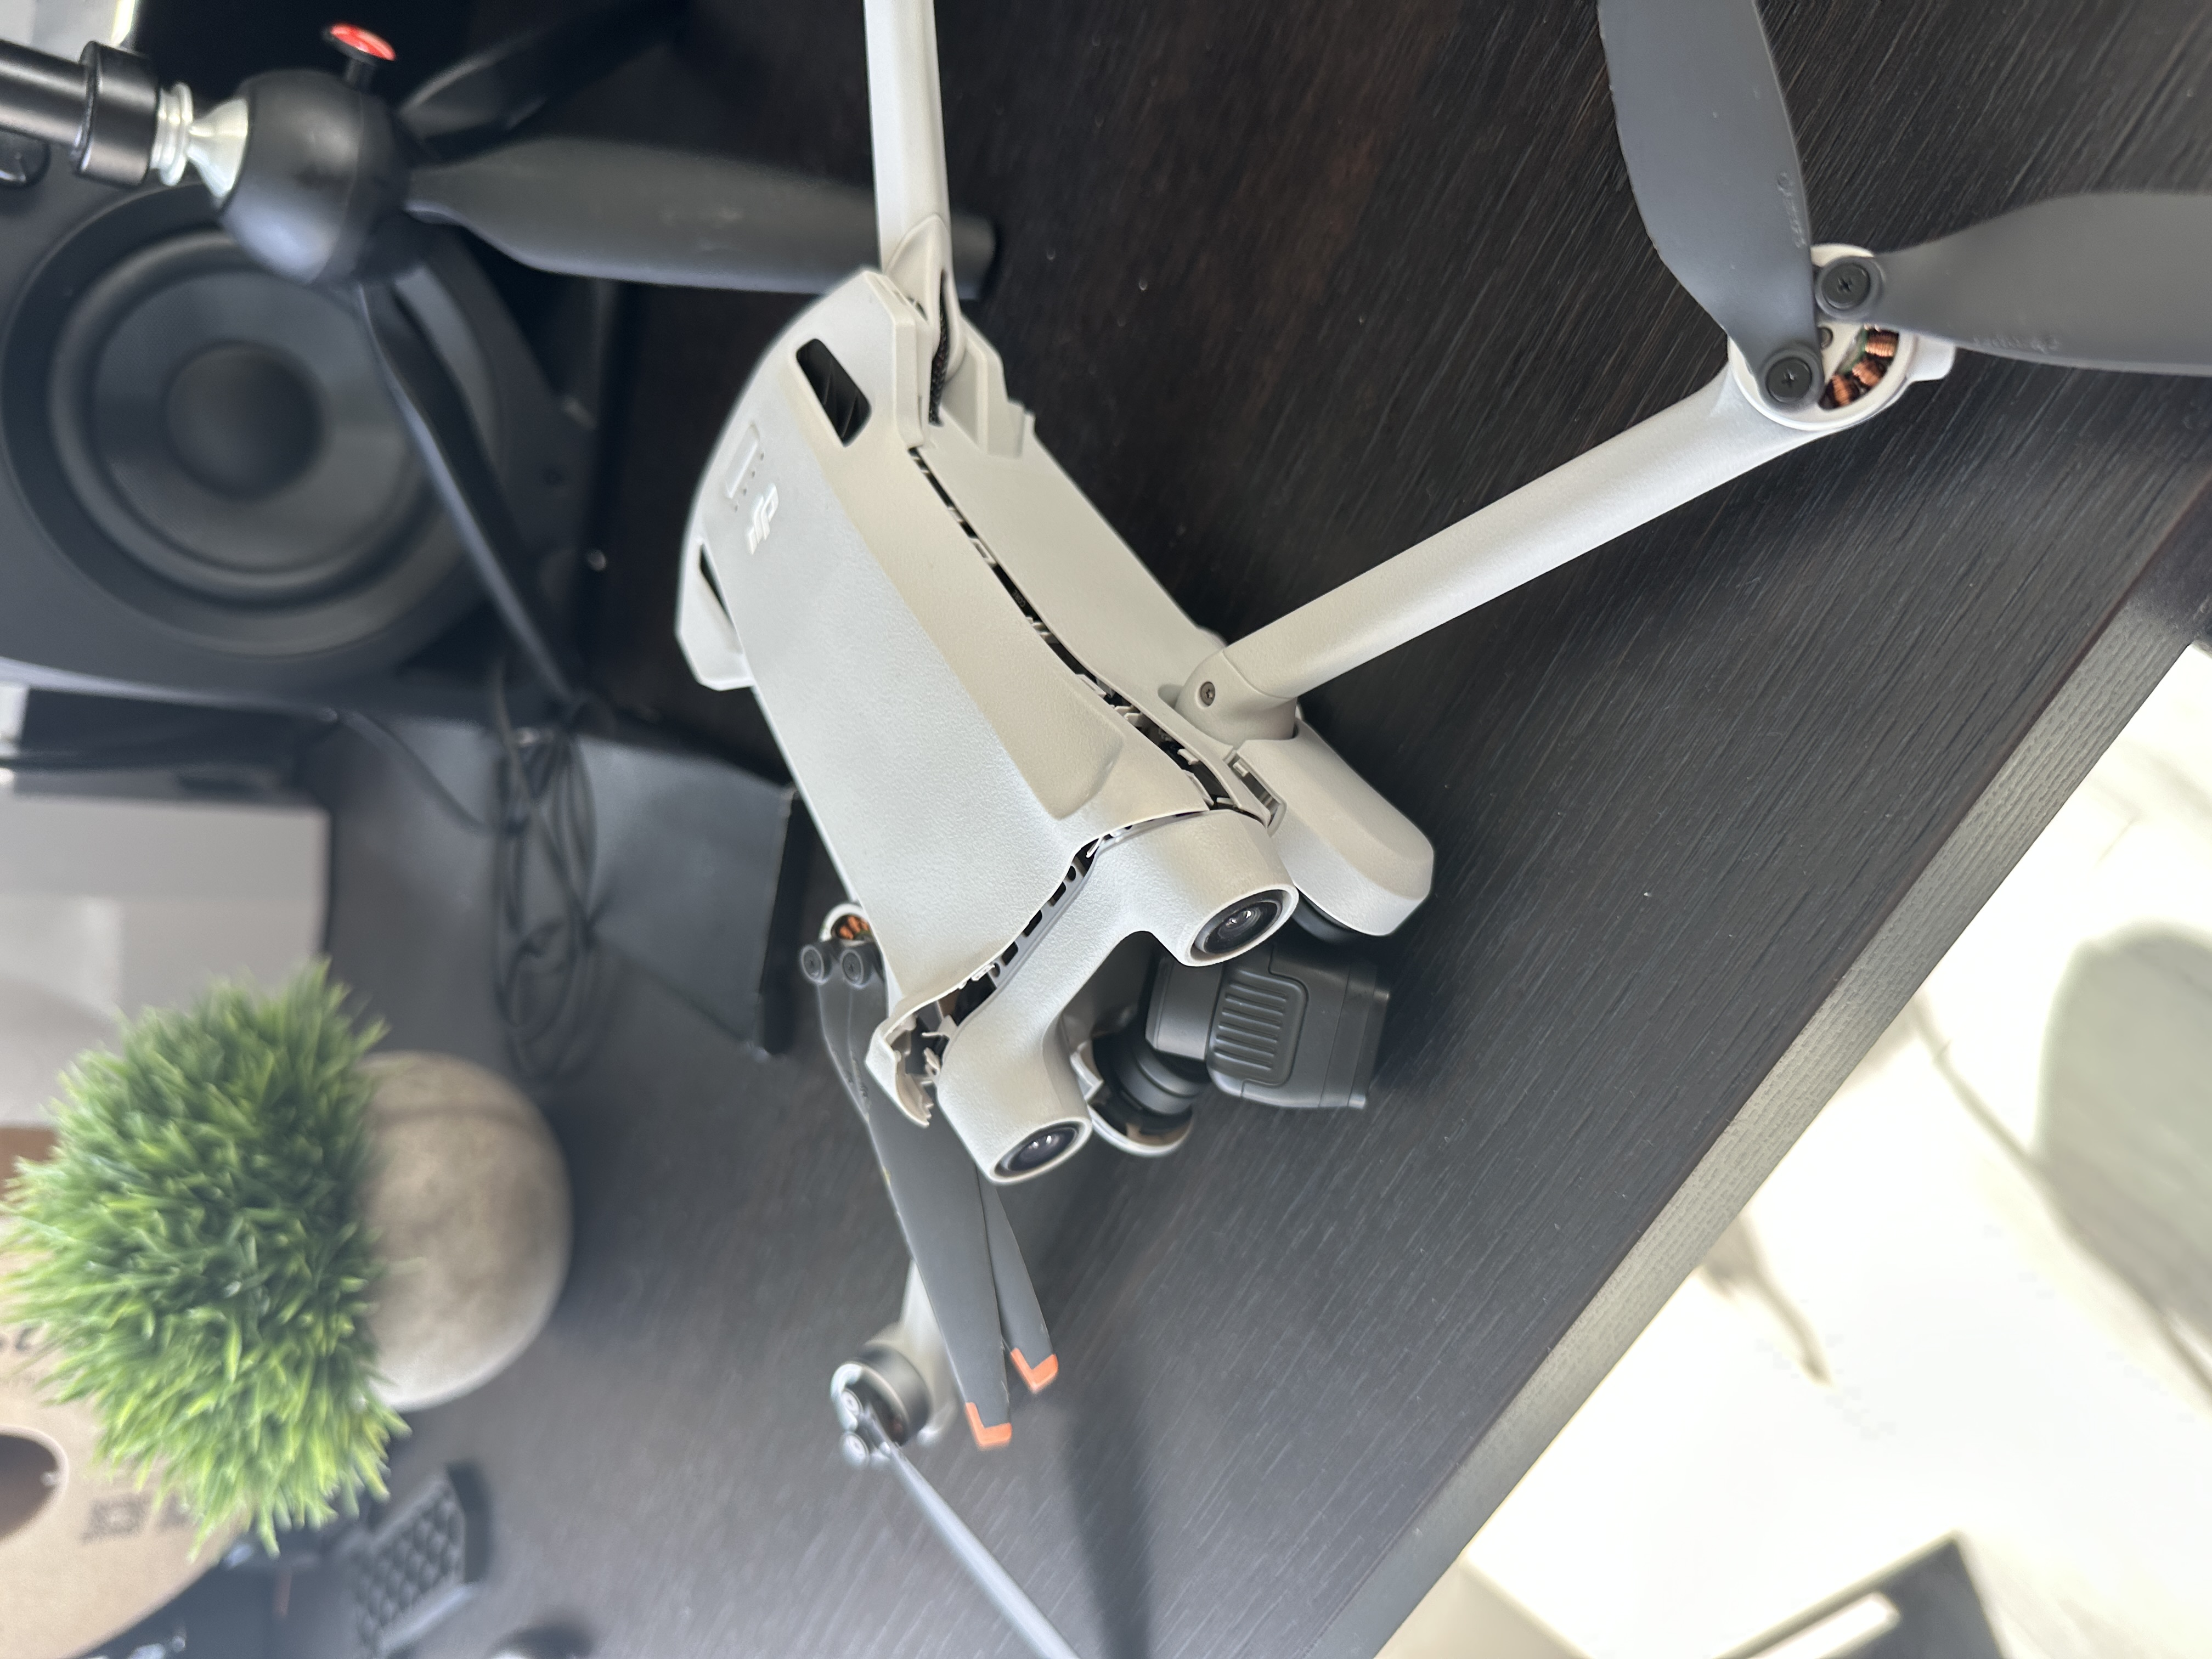
\includegraphics[width=8cm]{test.JPG}
  \caption{A colourful picture.}
  \label{Figure:figex}
\end{figure}
\newpage\textsl{}
This page shows you a subfigure example in \fref{Figure:figsubex}.
\begin{figure}[!htb]
  \centering
  \subfigure[The left caption]{
    
\includegraphics[width=4.2cm]{figure}
    \label{Figure:figsubex:left}
  }
  \subfigure[The right caption]{
    
\includegraphics[width=4.2cm]{figure}
    \label{Figure:figsubex:right}
  }
  \caption{A doubly colourful picture.}
  \label{Figure:figsubex}
\end{figure}

%% ----------------------------------------------------------------

\chapter{Conclusions} \label{Chapter:Conclusions}
It works.


%% ----------------------------------------------------------------

% \appendix
% \include{AppendixA}
\backmatter
\bibliographystyle{unsrt}
\bibliography{ECS}
\end{document}
%% ----------------------------------------------------------------
